\chapter{Experimental-Style Load Separation in WARP3D} \label{chap:load-separation-experimental}

%\section{Experimental-style Load Separation using WARP3D}

Following the methods of \cite{sharobeamlandes1994} for surface cracks in tension, the load separation technique was applied using the models' remote bending stress and CMOD.
Remote bending stress was used instead of applied force in order to compensate for the widely varying plate widths and lengths, since these could vary by a factor of 4--5, and cause similar changes in bending moment.
Similarly, the CMOD provided a much more useful localized displacement measure than the transverse displacement, since many of the shallower and narrower cracks cause little change to the plate's total compliance, and the plate width and length affects the transverse displacement under load.

Each of 20 plate geometries was run with boundary conditions large enough to cause substantial deformation as measured by the CMOD.
When the elastic component of CMOD was removed, the plastic CMOD values ranged from 0.020--0.037.
The stress-CMOD curve for the crack with dimensions \((\frac{a}{c}, \frac{a}{t})=(0.6, 0.8)\) was used as the reference curve, since it had the highest plastic CMOD value, making for easier interpolation of the \Sij separation parameter for the remaining curves.

The 20 \Sij curves ranged in value from 0.8--1.6. Since showing all 20 curves on one graph would be difficult to interpret, the family of curves is divided up by crack depth in \Crefrange{fig:Sij_at_02}{fig:Sij_at_08}.
As the earliest part of the plastic stress-CMOD curves tend to be less separable, a second set of graphs was constructed that excluded plastic CMOD values below 0.001.
Those figures are shown in \Crefrange{fig:Sij_spread_at_02}{fig:Sij_spread_at_08}.
These graphs also show the mean value of the separation parameter \Sij for each curve as a dashed line, and the deviation from that mean value.
The deviation from the mean \Sij values is given in \Cref{tab:Sij_percentage_grid}, where it can be seen that the separation parameters are consistent to within 0--3\% for \(0.6 \leq \frac{a}{t} \leq 0.8\), and within 1--6\% for \(0.2 \leq \frac{a}{t} \leq 0.4\).
As the \Sij values reported by \citeauthor{sharobeamlandes1994} were consistent to within 2\% for both surface cracks in tension and edge cracks in bending, the three-dimensional conditions and constraint effects present in surface cracks in bending have some influence on the load separation results.

\begin{figure}[tbp]
\centering
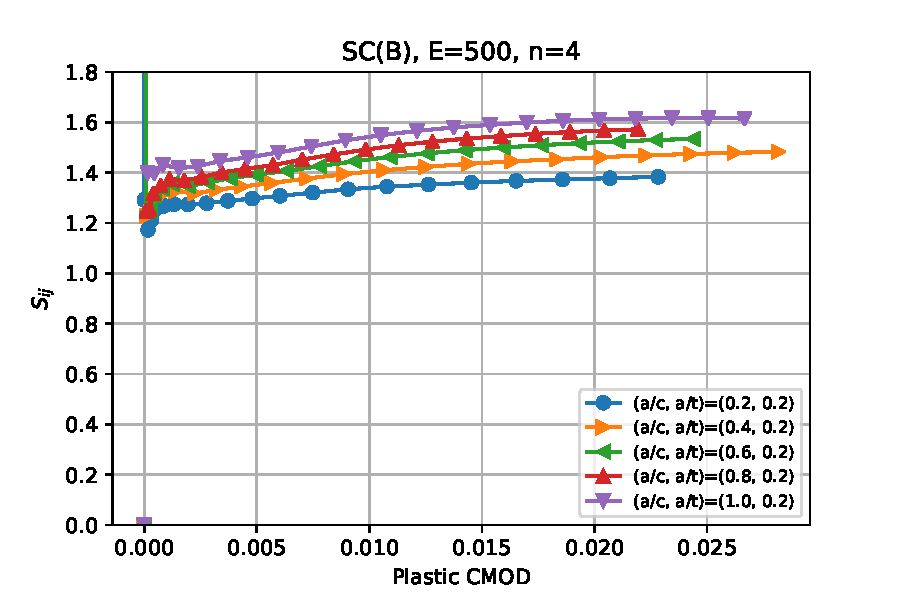
\includegraphics[width=0.8\columnwidth]{Sij_at_02}
\caption{Separation parameters for cracked plates in bending, \(\frac{a}{t}=0.2\) \label{fig:Sij_at_02}}
\end{figure}
\begin{figure}[tbp]
\centering
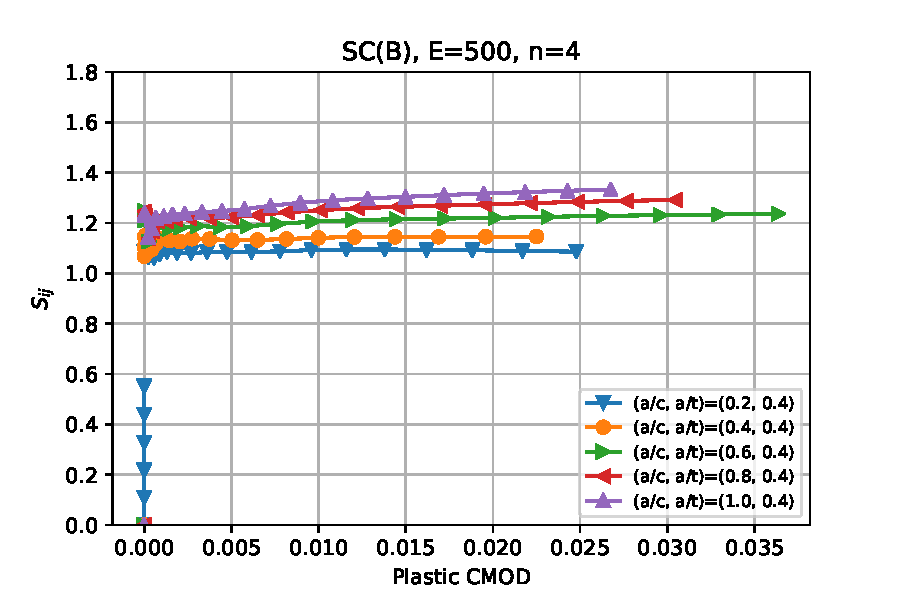
\includegraphics[width=0.8\columnwidth]{Sij_at_04}
\caption{Separation parameters for cracked plates in bending, \(\frac{a}{t}=0.4\) \label{fig:Sij_at_04}}
\end{figure}
\begin{figure}[tbp]
\centering
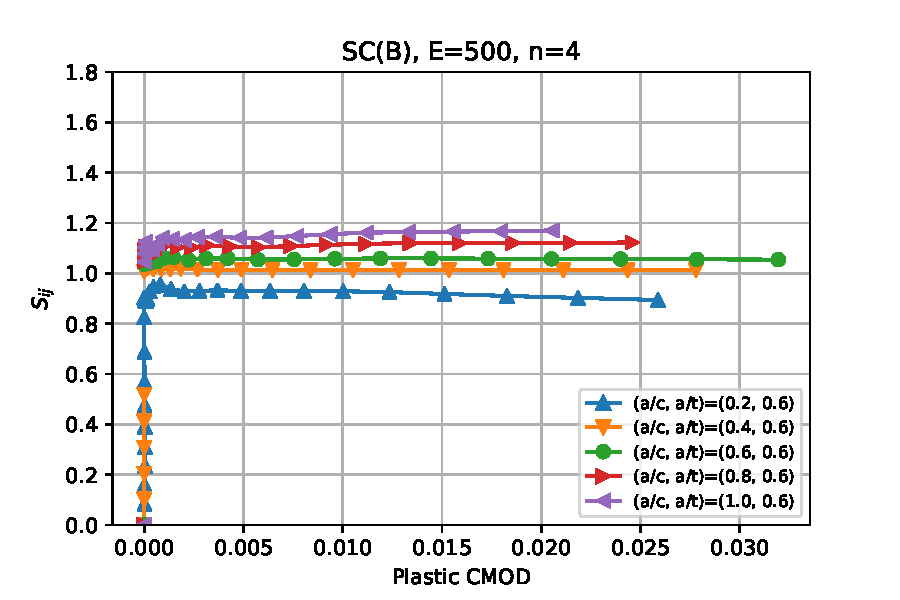
\includegraphics[width=0.8\columnwidth]{Sij_at_06}
\caption{Separation parameters for cracked plates in bending, \(\frac{a}{t}=0.6\) \label{fig:Sij_at_06}}
\end{figure}
\begin{figure}[tbp]
\centering
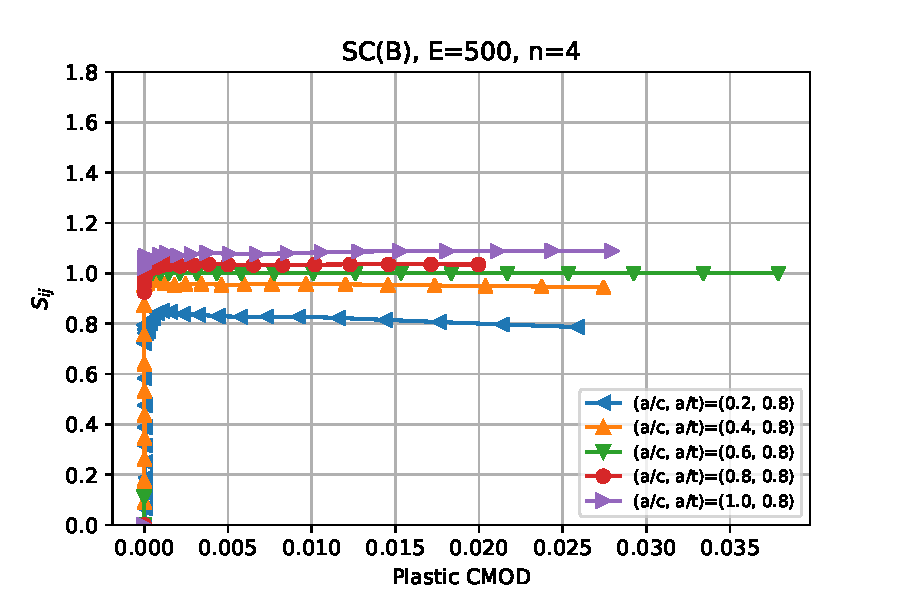
\includegraphics[width=0.8\columnwidth]{Sij_at_08}
\caption{Separation parameters for cracked plates in bending, \(\frac{a}{t}=0.8\) \label{fig:Sij_at_08}}
\end{figure}

\begin{figure}[tbp]
\centering
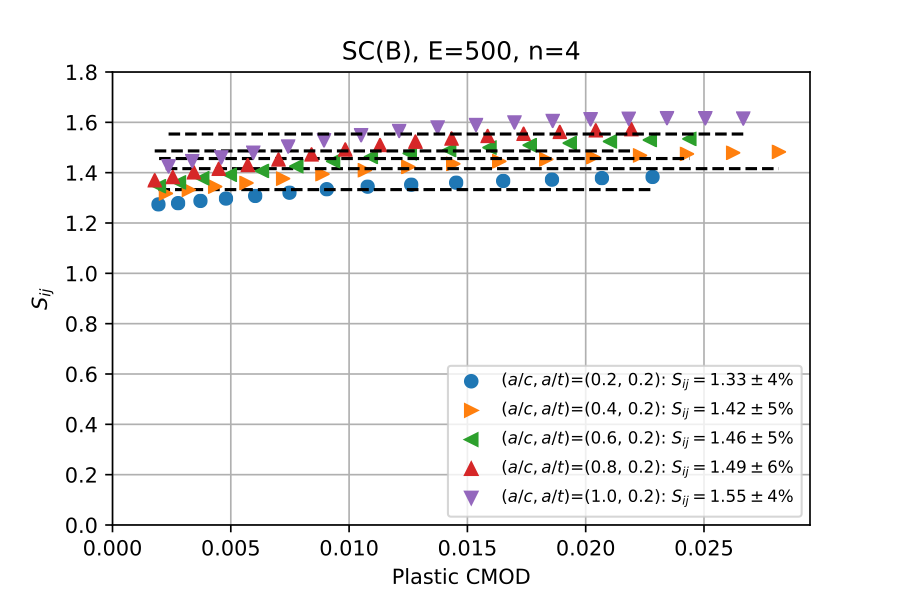
\includegraphics[width=0.8\columnwidth]{Sij_spread_at_02}
\caption{Variation of \Sij for cracked plates in bending, \(\frac{a}{t}=0.2\) \label{fig:Sij_spread_at_02}}
\end{figure}
\begin{figure}[tbp]
\centering
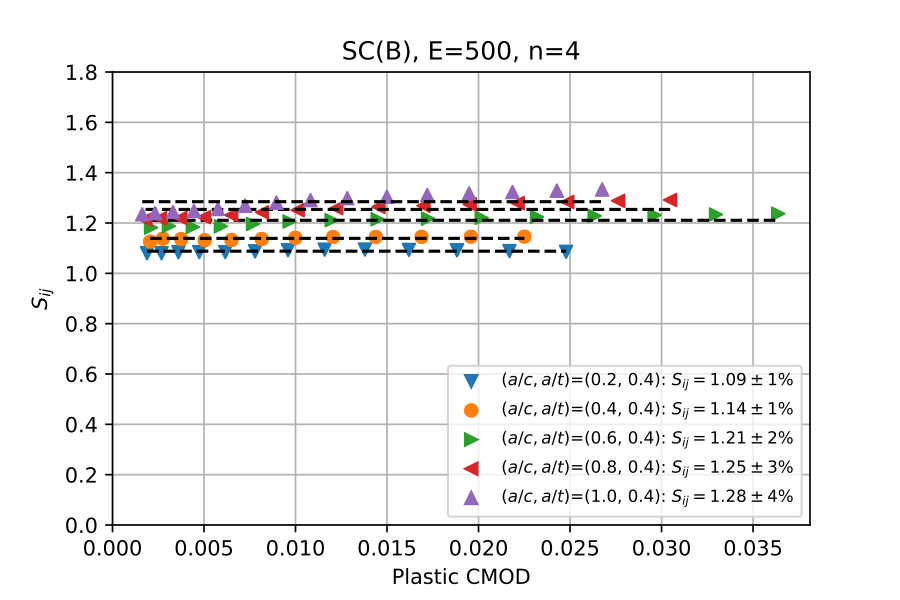
\includegraphics[width=0.8\columnwidth]{Sij_spread_at_04}
\caption{Variation of \Sij for cracked plates in bending, \(\frac{a}{t}=0.4\) \label{fig:Sij_spread_at_04}}
\end{figure}
\begin{figure}[tbp]
\centering
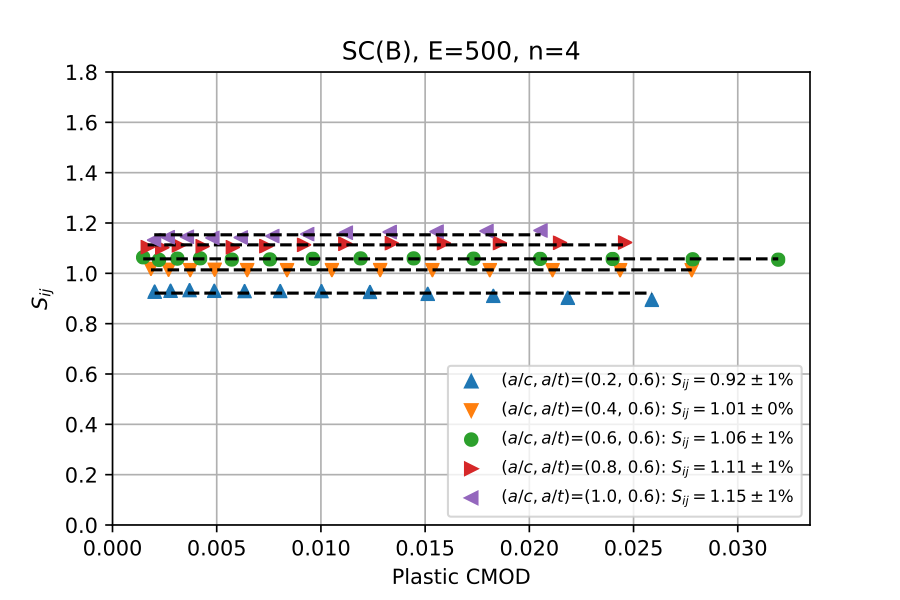
\includegraphics[width=0.8\columnwidth]{Sij_spread_at_06}
\caption{Variation of \Sij for cracked plates in bending, \(\frac{a}{t}=0.6\) \label{fig:Sij_spread_at_06}}
\end{figure}
\begin{figure}[tbp]
\centering
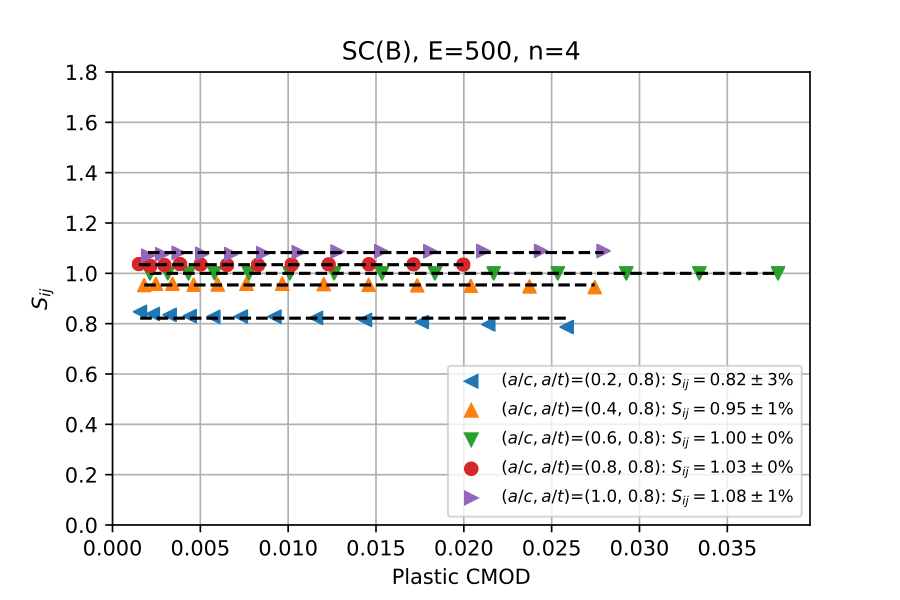
\includegraphics[width=0.8\columnwidth]{Sij_spread_at_08}
\caption{Variation of \Sij for cracked plates in bending, \(\frac{a}{t}=0.8\) \label{fig:Sij_spread_at_08}}
\end{figure}

\begin{table}
\caption{\label{tab:Sij_percentage_grid} Percent deviation of \Sij from mean value}
\centering
\begin{tabular}{SSSSS}
\toprule
& \multicolumn{4}{c}{\(\frac{a}{t}\)} \\
\multicolumn{1}{c}{\(\frac{a}{c}\)} & 0.2              & 0.4              & 0.6              & 0.8 \\ \cmidrule(lr){1-1} \cmidrule(lr){2-5}
0.2     & \SI{4}{\percent} & \SI{1}{\percent} & \SI{1}{\percent} & \SI{3}{\percent} \\
0.4     & \SI{5}{\percent} & \SI{1}{\percent} & \SI{0}{\percent} & \SI{1}{\percent} \\
0.6     & \SI{5}{\percent} & \SI{2}{\percent} & \SI{1}{\percent} & {N/A} \\
0.8     & \SI{6}{\percent} & \SI{3}{\percent} & \SI{1}{\percent} & \SI{0}{\percent} \\
1.0     & \SI{4}{\percent} & \SI{4}{\percent} & \SI{1}{\percent} & \SI{1}{\percent} \\ \bottomrule
\end{tabular}
\end{table}

Taking the ratio of the effective uncracked ligament to plate thickness in \cite{sharobeamlandes1994}
\begin{align}
\frac{b_e}{t} &= 1 - \frac{\pi a}{2t \left[ 2 + \frac{a/c}{a/t} \right]}
\end{align}
as a characteristic size of the crack, \Cref{fig:Sij_bet_full_E0500_n04} shows the variation of \Sij against the characteristic size.
When grouped by crack depth ratio $\frac{a}{t}$, it is clear that each group of cracks is follows a consistent trend, regardless of aspect ratio.
The curves for the shallower cracks ($0.2 \leq \frac{a}{t} \leq 0.4$) may even fall into a single larger trend, but the full set of curves does not lead to the generation of a single key curve like the one shown in \Cref{fig:sij-b-w}.
It is possible that an alternate measure of characteristic crack size could group the four curves closer together allowing a true single-specimen technique for bending, but development of this alternate measure has not yet been performed.
%Though the curves for \(\frac{a}{t} = 0.8\) and \(\frac{a}{t} = 0.6\) are similar, the ones for \(\frac{a}{t} = 0.4\) and \(\frac{a}{t} = 0.2\) are quite distinct, limiting the applicability of a single-specimen technique to this range of bending geometry.
\begin{figure}[tbp]
\centering
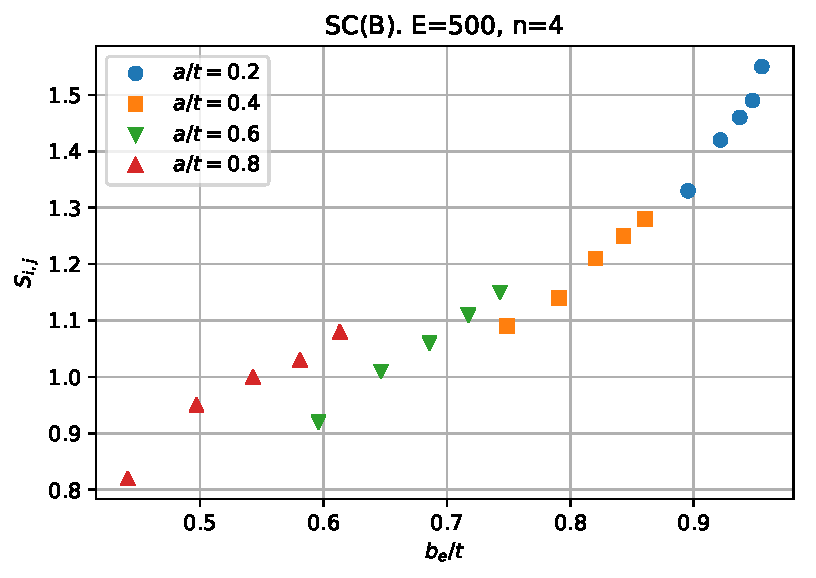
\includegraphics[width=0.8\columnwidth]{Sij_bet_full_E0500_n04}
\caption{Variation of \Sij versus effective uncracked ligament length ratio, \(0.2 \leq \frac{a}{t} \leq 0.8\) \label{fig:Sij_bet_full_E0500_n04}}
\end{figure}
%Even if the range of geometry is limited to a subset of values used in \cite{sharobeamlandes1994} (\(0.6 \leq \frac{a}{c} \leq 1.0, \quad 0.4 \leq \frac{a}{t} \leq 0.8 \)) in \Cref{fig:Sij_bet_subset_E0500_n04}, the curve for \(\frac{a}{t} = 0.4\) still deviates considerably from the curves for \(\frac{a}{t} = 0.6\) and \(\frac{a}{t} = 0.8\).
%An alternative development of \Sij using a measurement other than bending stress, or replacing the characteristic size with something other than the effective uncracked ligament may cause the curves to more closely align, but this development has not been carried out.
%It appears that for now, load separation for surface cracked plates in bending is only applicable to moderately or deeply-cracked bodies with relatively compact cracks (\(0.6 \leq \frac{a}{c} \leq 1.0, \quad 0.6 \leq \frac{a}{t} \leq 0.8\)).
%\begin{figure}[tbp]
%\centering
%\includegraphics[width=0.8\columnwidth]{Sij_bet_subset_E0500_n04}
%\caption{Variation of \Sij versus effective uncracked ligament length ratio, \(0.4 \leq \frac{a}{c} \leq 1.0\), \(0.6 \leq \frac{a}{t} \leq 0.8\) \label{fig:Sij_bet_subset_E0500_n04}}
%\end{figure}
